\section{Obstacles} \label{sec:obstacles}
    \subsection{Local Network Issues}
        An initial problem found when working with PBX software was configuring connections for the device hosting it and for the devices that are connected with it (e.g. smart phones and computers). As IP-PBX uses IP networks for its functionality, a single local network was used for testing the functionality of the Raspberry Pi, which the Pi itself and all machines running VoIP software were connected to, Eduroam. Eduroam is the primary wireless network used within the University of Alabama campus, with access points in each building, allowing devices across buildings to stay on one local area network. 
        
        This provided a few benefits to the experiment, most prominently allowing for VoIP calls to be made from greater distances (i.e. from a different building) while simplifying the process of connecting devices to the Raspberry Pi. However, an issue found with this was that Eduroam was not initially allowing the Pis to connect. An additional script was required to sign into the network as students. After the script was ran and the Pis rebooted, they could freely join the network afterward.
        
        \begin{figure}[htbp]
			\centerline{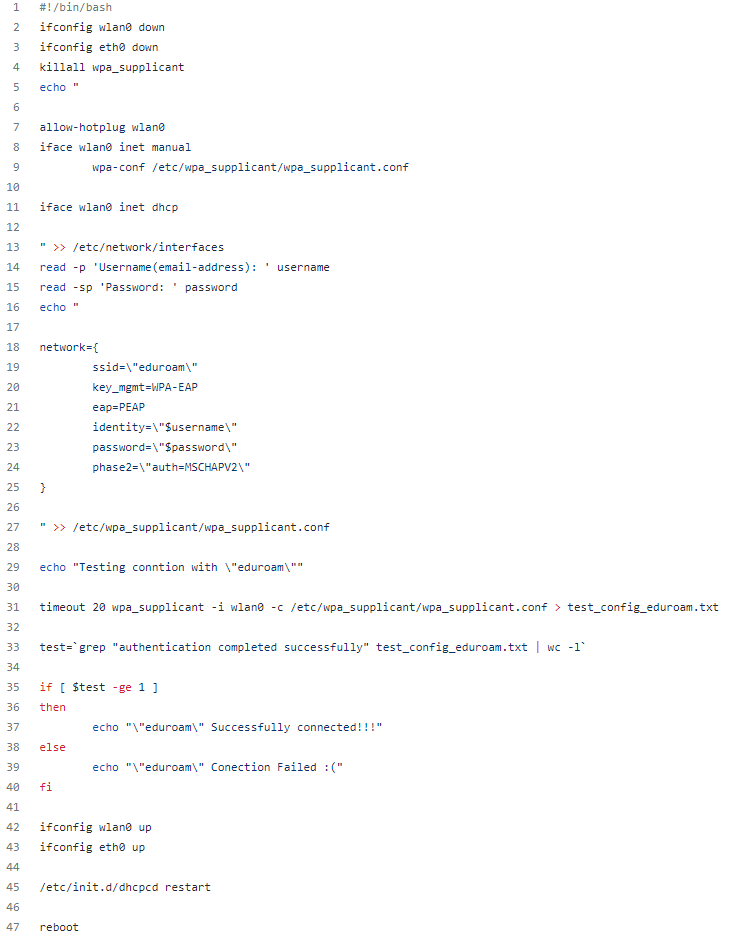
\includegraphics[width=8cm]{Images/experiment/eduroam.PNG}}
			\caption{Script used to join Eduroam network}
			\label{fig:edu-script}
		\end{figure}
		
		Another problem more central to the use of IP-PBX software is the complication of connecting remote devices to the Raspberry Pi. Within Eduroam, VoIP software only required the domain of the Raspberry Pi within the local area network to register on the IP-PBX software the Pi was running. However, if the device was on a different network, it proved incapable of finding the Pi as easily. There are a few possible explanations for this, such as there being a firewall blocking most traffic outside of Eduroam or NAT changing the IP of the Pi from outside Eduroam. Without the ability to make calls from different networks, making long distance VoIP calls proved to be quite limited, and the available tests for the Raspberry Pi were limited. While this issue may have been resolved with further research, it was ultimately decided that having all devices connect to Eduroam still allowed for enough trials to analyze the Pis functionality in running IP-PBX software.
		
	\subsection{Complexity of IP-PBX}
	    IP-PBX proved to be quite complex in setup and configuration. Asterisk PBX, a mature open-source implementation, was utilized. Initial compilation of Asterisk showed that there were many options on modules to be used, many of which were extraneous. After setup was done, the PBX needed to be further configured to allow for distinct users to be registered, to denote what should be done if a call was made to a certain number, and to dictate what kind of channel to use for SIP. Determining what configuration files needed to be used and changed and in what ways was a major obstacle in beginning the testing of the Raspberry Pi.
	    
	    \begin{figure}[htbp]
			\centerline{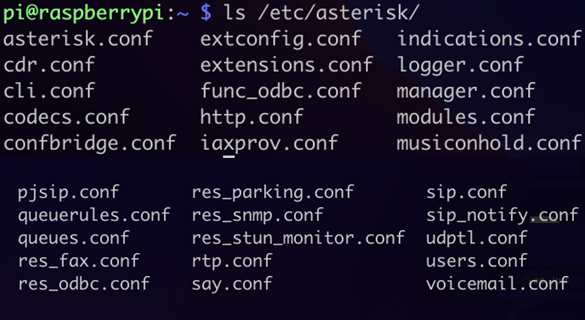
\includegraphics[width=8cm]{Images/experiment/config.png}}
			\caption{The configuration files for Asterisk PBX. Note that the majority of edits needed to be made to sip.conf and extensions.conf}
			\label{fig:conf}
		\end{figure}
		
	\subsection{Abundance of Third Party Software}
	    Many pieces of third party software needed to be utilized to conduct these tests, each adding more setup time and complication to the experiments. Asterisk PBX needed to be downloaded onto the Raspberry Pi to allow the Pi to provide IP-PBX services. Zoiper was needed to make VoIP calls and register devices on the Pi for IP-PBX services, with MicroSIP and Telephone needed to make additional calls, as Zoiper limits the number of free users. Wireshark was required to gather more information on the packets sent to and from the Pi while hosting calls to analyze its performance. Additionally, other services, such as SIP.US (used for SIP trunking) and Clumsy (used for network emulation) were considered for use until they were deemed unnecessary. The number of extraneous services utilized exacerbated the complexity of performing these experiments. enefits to the experiment, most prominently allowing for VoIP calls to be made from greater distances (i.e. from a different building) while simplifying the process of connecting devices to the Raspberry Pi. However, an issue found with this was that Eduroam was not initially allowing the Pis to connect. An additional script was required to sign into the network as students. After the script was ran and the Pis rebooted, they could freely join the network afterward.